\begin{figure}[t]
    \centering
    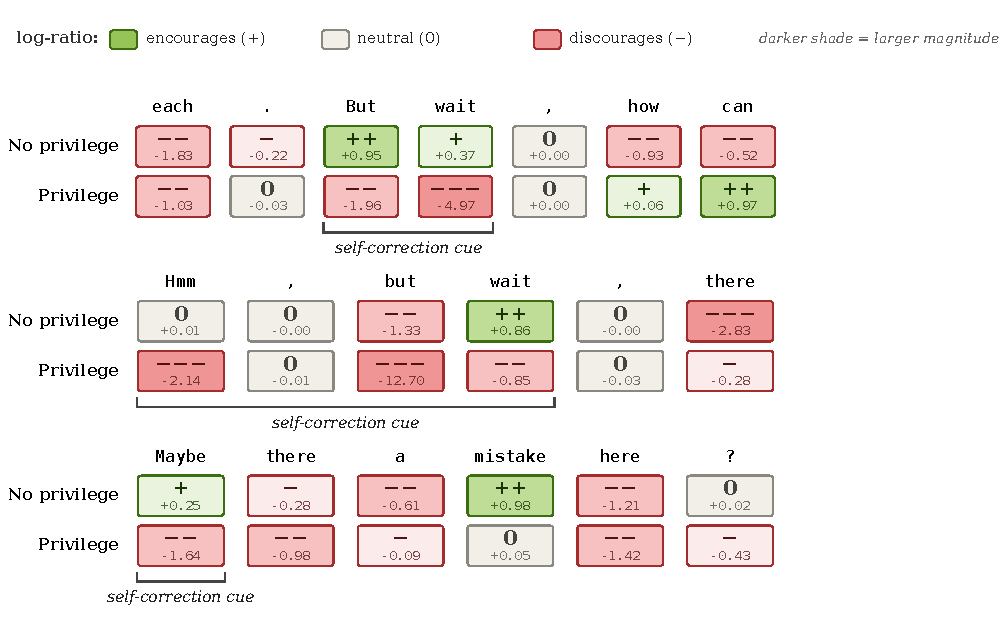
\includegraphics[width=0.95\linewidth]{figures/fig_privilege_flips_self_correction.pdf}
    \caption{\textbf{Privilege flips credit on self-correction cues, even
    when they lead to the correct answer.} Three windows from rollouts of
    a Qwen3-1.7B (Thinking) student trained against a Qwen3-8B (Thinking) teacher on
    OpenThoughts; the trajectory is identical under both teachers; only
    the teacher differs. Cells show the sign and magnitude of the
    per-token log-ratio
    $\log \pi_T(y_t \mid y_{<t}, x) - \log \pi_S(y_t \mid y_{<t}, x)$.
    \textbf{Top:} a rollout for \emph{``radius of a circle tangent to two
    concentric circles''} that ends at the wrong answer; privilege
    assigns negative advantage to \texttt{But wait} ($-1.96$, $-4.97$) and rewards the
    dismissive continuation \texttt{how can}. \textbf{Middle and bottom:}
    two windows from a rollout that reaches the \emph{correct} answer.
    Privilege still suppresses every self-correction cue, most extremely
    \texttt{but} ($-12.70$) and the hedge \texttt{Maybe} ($-1.64$). The
    pattern is consistent: the privileged teacher's positive credit moves
    away from the moments where the student notices something is off and
    onto the locally fluent continuation.}
    \label{fig:privilege-flips}
\end{figure}
